\documentclass[11pt]{beamer}
\usepackage[utf8]{inputenc}
\usepackage[T1]{fontenc}
\usepackage{amsmath}
\usepackage{amsfonts}
\usepackage{amssymb}
\usepackage{graphicx}
\usetheme{Copenhagen}

\newcommand{\indep}{\rotatebox[origin=c]{90}{$\models$}}

\begin{document}
	\author{Liu Xuefeng}
	\title{Probabilistic Graph Models}
	%\subtitle{}
	%\logo{}
	%\institute{}
	\date{\today}
	%\subject{}
	%\setbeamercovered{transparent}
	%\setbeamertemplate{navigation symbols}{}
	\begin{frame}[plain]
	\maketitle
\end{frame}

\begin{frame}
\frametitle{Bayesian Networks}
	\begin{itemize}
		\item The core of Bayesian network representation is a directed acyclic graph (DAG) G, whose
		nodes are the random variables in our domain and whose edges correspond, intuitively, to direct
		influence of one node on another.
	\end{itemize}
\end{frame}

\begin{frame}
\frametitle{Student Example}
\begin{figure}
	\centering
	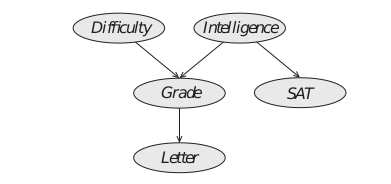
\includegraphics[width=0.7\linewidth]{pic/student}
%	\caption{}
	\label{fig:student}
\end{figure}
\[
P(I, D, G, S, L)=P(I)P(D)P(G|I, D)P(S|I)P(L|G)
\]
\end{frame}

\begin{frame}
\frametitle{Bayesian Network Structure}
A Bayesian network structure $G$ is a directed acyclic graph whose nodes represent random variables $x_1, x_2, \cdots, x_n$. 

Let $Pa_{x_i}^G$ denote the parents of $x_i$ in $G$, and $NonDescendants_{x_i}$ denote the variables in the graph that are not descendants of $x_i$. 

Then $G$ encodes the following set of conditional independence assumptions, called the local independencies:

\[
	(x_i \indep NonDescendants_{x_i} | Pa_{x_i}^G)
\]

\end{frame}

\begin{frame}
\frametitle{Indirect Connection}
\begin{figure}
	\centering
	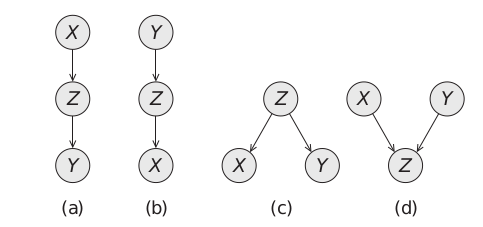
\includegraphics[width=0.7\linewidth]{pic/indirect}
	\label{fig:indirect}
\end{figure}

\begin{enumerate}
	\item [a] Indirect causal effect.
	\item [b] Indirect evidential effect.
	\item [c] Common cause.
	\item [d] Common effect.
\end{enumerate}

\end{frame}

\begin{frame}
\frametitle{d-separation}

\begin{definition}
Let $G$ be a BN structure, and $x_1-x_2-\cdots -x_n$ a trail in $G$. Let $Z$ be a subset of observed variables. The trail is active given $Z$ if 
\begin{itemize}
	\item Whenever we have a v-structure $x_{i-1}\rightarrow x_i \leftarrow x_{i+1}$, then $x_i$ or one of its descendants are in $Z$;
	\item no other node along the trail is in $Z$.
\end{itemize}
\end{definition}

\end{frame}


\begin{frame}
\frametitle{d-separation}

\begin{definition}
	Let $X, Y, Z$ be three sets of nodes in $G$. We say that $X$ and $Y$ are d-separated given $Z$, denoted $d-sep_G(X;Y | Z)$, if there is no active trail between any node $x \in X$ and $y \in Y$ given $Z$. We use $L(G)$ to denote the set of independencies that corresponds to d-separation:
	\[
		L(G)=\{(X \indep Y | Z): d-sep_G(X; Y| Z)\}
	\]
\end{definition}

\end{frame}

\begin{frame}
\frametitle{Misconception Example}
\begin{figure}
	\centering
	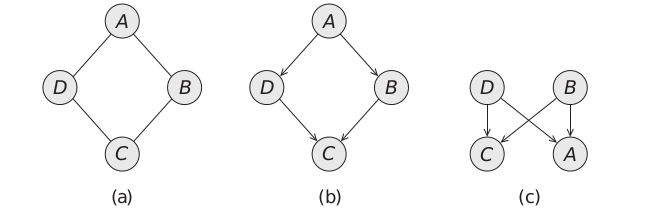
\includegraphics[width=0.7\linewidth]{pic/misconception}
	\label{fig:misconception}
\end{figure}

\begin{itemize}
	\item $(B \indep D | \{A, C\})$
	\item $(A \indep C | \{B, D\})$
\end{itemize}

\end{frame}

\begin{frame}
\frametitle{Markov Network}
\begin{definition}
	Let $D$ be a set of random variables. We define a factor $\phi$ to be a function from $Val(D)$ to $R$. The set of variables $D$ is called the scope of the factor and denoted $Scope[\phi]$.
\end{definition}

\begin{definition}
	Let $X$, $Y$, $Z$ be three disjoint sets of variables, and let $\phi_1(X, Y)$ and $\phi_2(Y, Z)$ be two factors. We define the factor product $\phi_1 \times \phi_2$ to be factor $\phi: Val(X, Y, Z) \rightarrow R$ as follows:
	\[
		\phi(X, Y, Z)=\phi_1(X, Y) \phi_2(Y, Z).
	\]
\end{definition}
\end{frame}

\begin{frame}
\frametitle{Misconception Example}
\begin{figure}
	\centering
	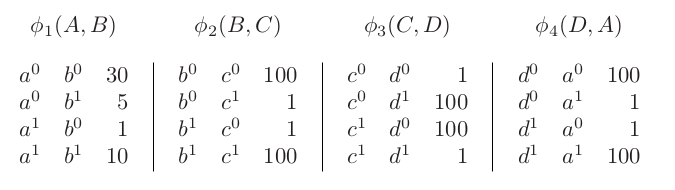
\includegraphics[width=0.7\linewidth]{pic/factor}
%	\caption{}
	\label{fig:factor}
\end{figure}
\begin{figure}
	\centering
	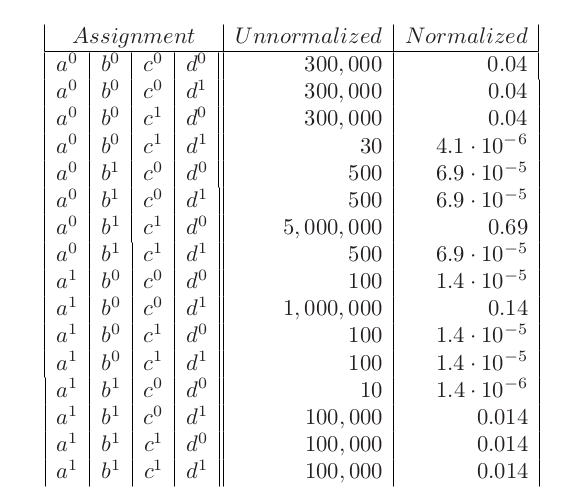
\includegraphics[width=0.7\linewidth]{pic/joint}
%	\caption{}
	\label{fig:joint}
\end{figure}


\end{frame}



\end{document}